\chapter{Project}
This section will discuss the entities and requirements evaluated from the proposal.

\section{Requirements}
From the written proposal, some requirement were evaluated:
\begin{enumerate}
\item The system should be able to run queries in the database currently employed at the institution.\label{req:multidb}
\item Users can only run queries in which they have Permission to.\label{req:permission}
\item Query commands may be longer than 30 lines long.\label{req:longquery}
\item Running a Query yields a table that can be downloaded.\label{req:download}
\item No \gls{SQL} knowledge is needed to execute a Query.\label{req:noknowledge}
\item The system enables the insertion of new Queries.\label{req:addquery}\todo{dependendo do perfil do utilizador??}
\end{enumerate}

Given the context and the objective of this project, four entities were found to play a significant role:
\begin{description}
\item[Database]
  Where a Query is run.
\item[Query]
  A script that is run in a Database and gather information into a single table.
\item[Permission]
  The binding between Users and Queries.
\item[User]
  Either an user or an Administrator that interacts with the system.
\end{description}

Use cases were also identified:
\begin{description}
\item[User]
  \begin{enumerate}
  \item Execute a query
  \end{enumerate}
\item[Administrator]
  \begin{enumerate}
  \item \gls{CRUD} Query
  \item \gls{CRUD} Permission
  \item \gls{CRUD} Directory
  \item Associate User and Permission
  \end{enumerate}
\end{description}

\todo{importante mas nao sei onde por ainda}
Queries must be associated to one Permission.
Users may have more than one permission.
The system must authenticate using the institute's centralized directory server.
An Administrator can manage the system by altering everything that is in the scope of this system.

Permissions is a central piece of this system. It's what associates users with information.
Permissions follow a hierarchy. There is a root Permission whose path is simply ``/'' and it's parent is itself.
There are two roles that any given user may be assigned to, either Administrator or User.

\section{Class Diagram}
\todo{de alguma forma, chegou nesse diagrama}
\begin{figure}
  \centering
  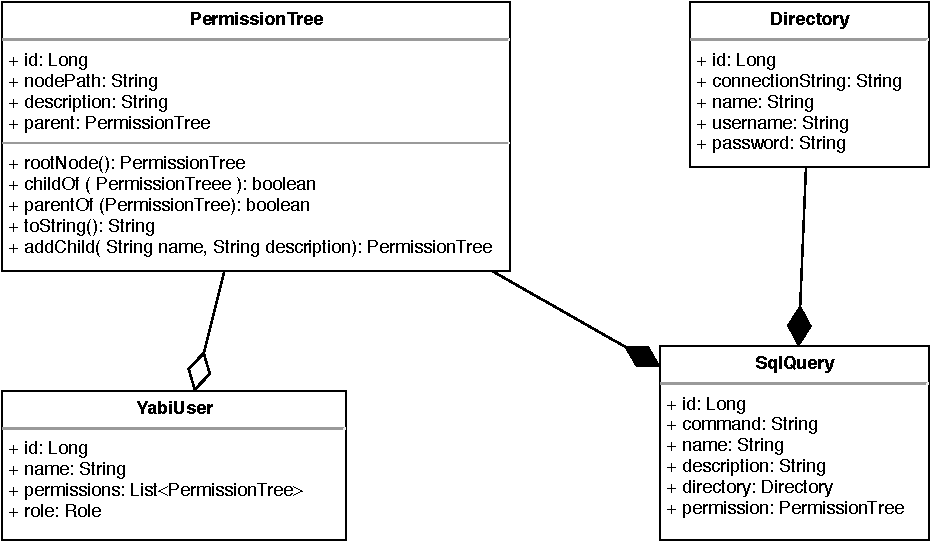
\includegraphics[width=.5\textwidth]{images/diagramas/class}
  \caption{Class diagram}\label{fig:classdiagram}
\end{figure}

\section{Template Sb-Admin-Material}
\section{Multi-Database Support}

Even though the context in which the application described in this document will be primarily accessing Oracle databases, support for other databases was added to broaden its usefulness.

As far as the project for implementing this feature goes, Figure\ref{fig:multidbproj} hopefully describes the process. When a request to run a given Query arrives,
